\documentclass[letterpaper, 12pt, oneside]{article}%´
\usepackage{amsmath}%paquete para escribir expresiones matemámaticas
\usepackage{graphicx}%paquete para poder incluír imagenes en el documento
\usepackage{xcolor} %paquete de LaTex para poder poner otro texto
\graphicspath{{Imagenes/}}%directorio de la imagen, este lo cambian por el directorio en el que ustedes guardaron su imagen 1.png
\usepackage[utf8]{inputenc} %para poder poner acentos

	\title{\Huge Taller de Herramientas Computacionales}
	%\title{\Huge \colorbox{magenta}{Taller de Herramientas computacionales}} %De esta forma con colorbox pone el texto dentro de una "caja" de color.
	\author{Josué Artemio Hernández Rodríguez}%autor del escrito
	\date{11/01/19}%fecha del escrito

\begin{document}%inicia el documento
\maketitle
%\vfill %Para rellenar el espacio y colocar hasta abajo de la pagina el siguiente texto, imagen.
\begin{center}%inicia centrado
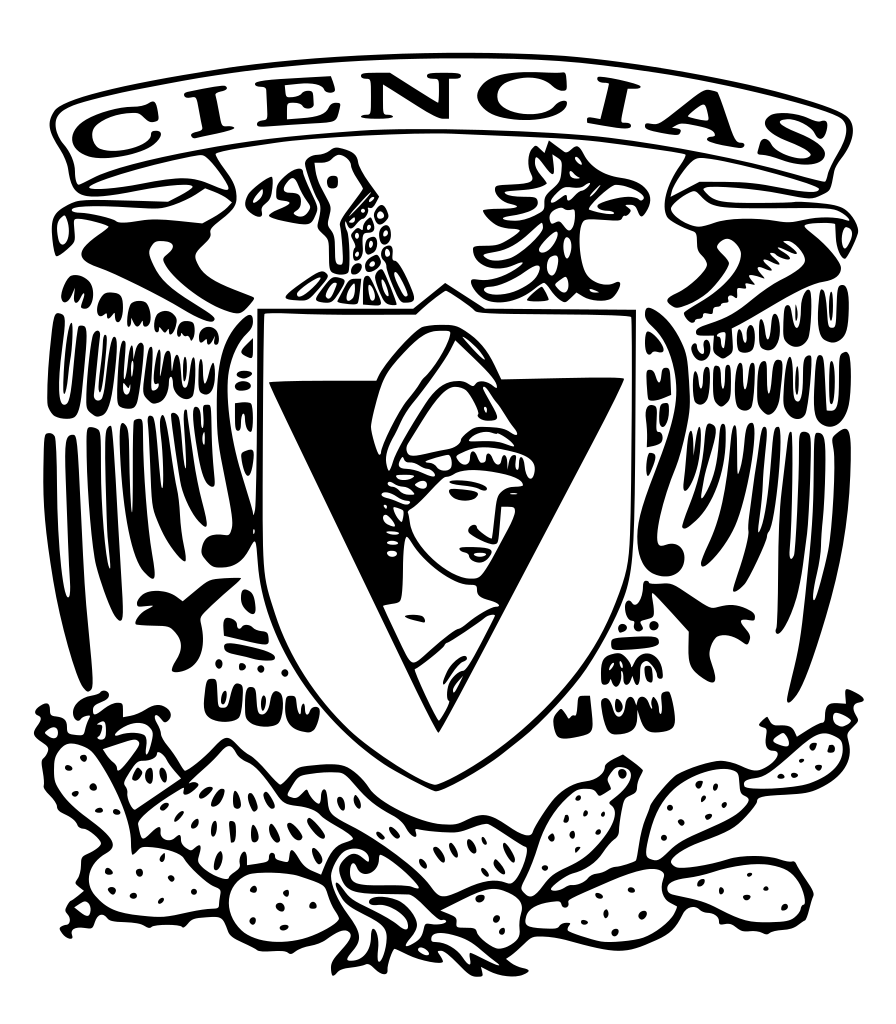
\includegraphics[scale=0.2]{2.png}%del lado izquierdo se muestra el tamaño de la imagen, del derecho se escribe el nombre de la imagen a incluir en el texto
\end{center}%termina el centrado para la imagen
\newpage%crea una nueva página

\title{\Huge Trabajando con python y LaTeX\\}%titulo2 \\ sirven para saltar una linea.

Lo que vimos en clase fue:%letras de color azul
\begin{enumerate}%Inicio de númeración para enlistar las cosas vistas en clase.
	\item Algunos conceptos y software utilizado en clase%item sirve enlistar el elemento, este es el primer elemento enumerado.
		\begin{itemize}
			\item '''texto''' se utiliza para realizar un comentario con multilinea y para que aparezcan en pantalla basta usar antes el comando print 			
			\item Scrip: Son instrucciones de Bash o en otro lenguaje que siguen una secuencia especifica			
			\item Palabras reservadas en python estan reservadas para el lenguaje de ese interprete, es decir no puedes nombrar ninguna variable con esas secuencias de letras, por ejemplo: print, import, etc.
			\item Un modulo en python es una secuencia de funciones.
		\end{itemize}
	
	\item Comandos de python%Segundo elemento enumerado.
	\begin{itemize}%comienza el enlistado pero itemize a diferencia de enumerate enlista sin un orden secuencial (es decir no utiliza números, ni letras)
		\item El simbolo \% en python sirve para denotar que se va sustituir por una variable, y en LaTex se usa para realizar comentarios.
		\item se utiliza "\%g" para expresar el flotanto en su forma mas corta
		\item Si tengo una variable con una cadena y quiero mostra su contenido con print, debo poner print '\%s' \%(c1)
		\item se utiliza "\ n" para denotar que hay un espacio entruna linea y otra
		\item Se utiliza "\%f" para expresar un numero en forma flotante
		\item Se utiliza math.sqrl para realizar una raíz cuadrada
		\item Se utiliza math.pow para raices en cualquier base, por ejemplo: math.pow (9,1.0/3), que significa, la raiz cubica de 9
		
				
	\end{itemize}%finaliza enlistado con itemize
	\item Comandos de LaTeX y comandos en terminal para instalar paquetes necesarios
		\begin{enumerate}
			\item Para instalar texstudio basta con escribir en la terminal "dnf install texstudio"
			\item Que significa la estructura de LaTeX
			\begin{enumerate}
				\item documentclass[]{} Expecificaciones del documento
				\item usepackage{amsmath} Paquete para escribir expresiones matemáticas
				\item usepackage{graphicx} Paquete para poder incluír imagenes en el documento
				\item usepackage{xcolor} Paquete de LaTex para poder poner otro texto
				\item graphicspath{{Imagenes/}} Directorio de la imagen, este lo cambian por el directorio
				\item usepackage[utf8]{inputenc} Sirve para poder poner acentos
				\item title{} Le agrega un titulo a nuestro texto
				\item author{} Autor del escrito
				\item date{11/01/19} Fecha
				\item begin{document} Inicia el documento
				\item end{document} Finaliza el documento
				\item maketitle Hace una portada a nuestro documento
				\item begin{center} Inicia el centrado de un texto o un objeto/imagen
				\item end{center} Finaliza el centrado
				\item newpage Crea una nueva página
				\item title{} Pone un titulo
				\item Huge o huge Pone letras grandez o muy grandes
				\item begin{enumerate} Inicio de númeración para enlistar las cosas vistas en clase y finaliza con end{enumerate} y finaliza con end{enumerate}
				\item begin{itemize} enlista y finaliza con end{itemize}
				\item item enumera, es parte de begin{enumerate} o begin{itemize}
				\item textbf Pone letras en negrita
				
			\end{enumerate}
			
		\end{enumerate}
	\item \textbf{Tarea}
		\begin{itemize}
			\item Hacer un modulo del programa en python que hicimos de tarea
			\item Realizar un resumen por cada clase en LaTeX
			\item Realizar preguntas
			
		\end{itemize}
	Buscar un problema de física que requiera la aplicacion de una fórmula para resolverlo
		
	
\end{enumerate}%finaliza el enlistado principal
	


\end{document}%termina el documento